%%%%%%%%%%%%%%%%%%%%%%%%%%%%%%%%%%%%%%%%%
% Stylish Article
% LaTeX Template
% Version 2.1 (1/10/15)
%
% This template has been downloaded from:
% http://www.LaTeXTemplates.com
%
% Original author:
% Mathias Legrand (legrand.mathias@gmail.com) 
% With extensive modifications by:
% Vel (vel@latextemplates.com)
%
% License:
% CC BY-NC-SA 3.0 (http://creativecommons.org/licenses/by-nc-sa/3.0/)
%
%%%%%%%%%%%%%%%%%%%%%%%%%%%%%%%%%%%%%%%%%

%----------------------------------------------------------------------------------------
%	PACKAGES AND OTHER DOCUMENT CONFIGURATIONS
%----------------------------------------------------------------------------------------

\documentclass[fleqn,10pt]{SelfArx} % Document font size and equations flushed left

\usepackage[italian]{babel} % Specify a different language here - english by default

\usepackage{float}
%----------------------------------------------------------------------------------------
%	COLUMNS
%----------------------------------------------------------------------------------------

\setlength{\columnsep}{0.55cm} % Distance between the two columns of text
\setlength{\fboxrule}{0.75pt} % Width of the border around the abstract

%----------------------------------------------------------------------------------------
%	COLORS
%----------------------------------------------------------------------------------------

\definecolor{color1}{RGB}{0,0,90} % Color of the article title and sections
\definecolor{color2}{RGB}{0,20,20} % Color of the boxes behind the abstract and headings

%----------------------------------------------------------------------------------------
%	HYPERLINKS
%----------------------------------------------------------------------------------------

\usepackage{hyperref} % Required for hyperlinks
\hypersetup{hidelinks,colorlinks,breaklinks=true,urlcolor=color2,citecolor=color1,linkcolor=color1,bookmarksopen=false,pdftitle={Title},pdfauthor={Author}}

%----------------------------------------------------------------------------------------
%	ARTICLE INFORMATION
%----------------------------------------------------------------------------------------

\JournalInfo{Progetto di \textit{Foundation of Probability and Statistics}, Università degli Studi di Milano Bicocca} % Journal information
\Archive{Anno Accademico 2019-20} % Additional notes (e.g. copyright, DOI, review/research article)

\PaperTitle{Spotify Dataset - Analisi delle tracce musicali e previsione della popolarità} % Article title

\Authors{Riccardo Cervero\textsuperscript{1}} % Authors
\affiliation{\textsuperscript{1}\textit{794126, Dipartimento di Informatica, Sistemistica e Comunicazione}} % Author affiliation

\Keywords{Inferenza - Previsione} 
\newcommand{\keywordname}{Keywords} 

%----------------------------------------------------------------------------------------
%	ABSTRACT
%----------------------------------------------------------------------------------------

\Abstract{Durante l'ultimo ventennio, grazie allo sviluppo di applicazioni \textit{web} per l'ascolto sempre più efficienti, la fruizione di contenuti musicali ha mostrato un'importante e rapida evoluzione, permettendo all'utente di accedere a qualsiasi brano - o qualunque versione dello stesso - in brevissimo tempo e, nella maggior parte dei casi, gestire autonomamente un archivio di tracce e artisti preferiti. L'industria discografica ha saputo sfruttare tale progresso, non soltanto incrementando il volume di distribuzione e di campagne promozionali, ma anche approfondendo quantitativamente e qualitativamente le tendenze d'ascolto di un pubblico catalogato. Moderne piattaforme offrono, infatti, la possibilità di estrarre ed analizzare una vasta varietà di parametri acustici e non, cosicché il produttore possa dedurre quali sono le caratteristiche più ricercate dal pubblico in un determinato momento e aumentare così la popolarità della traccia. È il caso, ad esempio, di \textit{Spotify}. Questo progetto, pertanto, ha come obiettivo l'analisi statistica delle caratteristiche qualitative e quantitative registrate da \textit{Spotify} in un \textit{database} di tracce disponibili all'interno del proprio servizio di \textit{streaming musicale}. Più precisamente, nella seconda e terza sezione verranno esaminate le variabili,  testata la loro reciproca connessione - di tipo lineare o non - e calcolate stime intervallari per le rispettive medie o proporzioni fra le modalità. Infine, nelle due successive sezioni, verranno esposti i risultati dei modelli di regressione lineare - sia semplice che multivariata - per la previsione della popolarità del brano e della positività emotiva da esso trasmessa.} 

%----------------------------------------------------------------------------------------

\begin{document}

\flushbottom % Makes all text pages the same height

\maketitle % Print the title and abstract box

\tableofcontents % Print the contents section

\thispagestyle{empty} % Removes page numbering from the first page

%----------------------------------------------------------------------------------------
%	ARTICLE CONTENTS
%----------------------------------------------------------------------------------------

\section{Caso di studio}
I dati esaminati nell'ambito di questo progetto provengono dal database di \textit{Kaggle} "Spotify Dataset"\footnote{Il link da cui è possibile scaricare il database "Spotify Dataset" è \href{https://www.kaggle.com/yamaerenay/spotify-dataset-19212020-160k-tracks}{\texttt{/kaggle/spotify-dataset-160k-tracks}}.}, che raccoglie un totale di 19 caratteristiche acustiche e qualitative relative a 169909 tracce, rese disponibili sulla piattaforma \textit{Spotify for Developers}\footnote{La documentazione della piattaforma \textit{Spotify for Developers} è disponibile al link \href{https://developer.spotify.com}{\texttt{developer.spotify.com}}.}\\
Le variabili oggetto di studio\footnote{La descrizione ufficiale delle variabili è disponibile ai link \href{https://developer.spotify.com/documentation/web-api/reference/tracks/get-audio-features/}{\texttt{developer.spotify/audio-features}} e \href{https://developer.spotify.com/documentation/web-api/reference/tracks/get-track/}{\texttt{developer.spotify/get-track}}.} corrispondono alle seguenti grandezze:
\begin{itemize}
    \item \textit{Acousticness} - o "acusticità" , è misura numerica - fra 0 e 1 - della confidenza con cui è possibile definire "acustica" una traccia: se 1, indica massima certezza nell'affermare che il brano sia stato prodotto senza strumenti elettronici
    \item \textit{Danceability} è il grado di ballabilità calcolato fra 0 e 1, come combinazione di vari elementi musicali, fra cui la stabilità del ritmo e il tempo
    \item \textit{Duration} è la durata del brano in millisecondi
    \item \textit{Energy} rappresenta la percentuale di intensità della traccia, sulla base di elementi percettivi quali sonorità e timbro
    \item \textit{Explicit} è variabile binaria che rileva la presenza o meno di contenuto esplicito
    \item \textit{Instrumentalness} misura, fra 0 e 1, l'assenza di contenuto vocale: più il valore si avvicina a 1, maggiore è la confidenza con cui si definisce "strumentale" la traccia
    \item \textit{Key} registra la stima della chiave complessiva della traccia, codificata in un valore numerico compreso fra 0 (Do) e 11 (Si)
    \item \textit{Liveness} rileva la presenza di un pubblico udibile nella registrazione, definendone la probabilità: se superiore a 0,8, fornisce una forte evidenza che la traccia sia stata registrata dal vivo
    \item \textit{Loudness} è il volume complessivo in decibel, fra -60 e circa 4
    \item \textit{Mode} è la variabile binaria circa la tonalità del brano: 1 se maggiore, 0 se minore
    \item \textit{Speechiness} indica la presenza di parlato: maggiore la somiglianza tra la traccia e un discorso - come nel caso del genere \textit{rap} -, maggiore la vicinanza del valore a 1
    \item \textit{Tempo} è il ritmo misurato in battiti al minuto (bpm)
    \item \textit{Valence} definisce il grado di positività emotiva trasmessa dal brano, tra 0 e 1
    \item \textit{Year} è l'anno di uscita del brano, dal 1921 al 2020
    \item \textit{Popularity} è una variabile intera compresa fra 0 e 100, che esprime il grado di popolarità del brano, calcolato a partire dal numero totale di riproduzioni su \textit{Spotify} e da quanto sono recenti tali ascolti: in generale, tracce riprodotte molto frequente durante l'anno corrente avranno un valore di popolarità molto elevato
\end{itemize}
Tali colonne verranno presentate singolarmente nei diversi paragrafi delle Sezioni \ref{cqual} e \ref{cquant}. In particolare, la popolarità verrà considerata come principale variabile \textit{target} nell'ambito della definizione di modelli di regressione.\\
\subsection{Pre-processing}
Il dataset originale non presentava alcun valore mancante, e le uniche operazioni di \textit{pre-processing} hanno implicato il raggruppamento delle modalità dell'anno di pubblicazione in classi di decennio (Sezione \ref{year}) e la rimozione delle variabili poco interessanti per l'obiettivo di analisi statistica: l'identificatore primario della traccia, il titolo, la lista di artisti accreditati e la data di pubblicazione. In particolare, la data di pubblicazione \textit{Release\_date} si manifestava in formato YYYY-MM-DD soltanto nel 70\% dei casi, mentre la restante parte riportava soltanto l'anno, così come la colonna \textit{Year}. Non potendo risalire al mese e al giorno, si è preferito eliminare \textit{Release\_date}.
%------------------------------------------------
\section{Analisi dei caratteri qualitativi}\label{cqual}
\subsection*{Variabile \textit{Year}}\label{year}
Le osservazioni del database "Spotify Dataset" sono distribuite con una certa coerenza fra i singoli anni - dal 1921 al 2020: le frequenze relative delle modalità di \textit{Year} sono identiche o comunque molto simili a 0.012 - che corrisponde alla frequenza relativa massima - in 73 anni su 100. Osservazioni meno numerose sono comprensibilmente relative agni anni precedenti al 1947. Perciò, la distribuzione di questa variabile qualitativa ordinale, oltre ad essere multimodale, può anche essere definita estremamente eterogenea: infatti, la mutabilità del fenomeno, misurata dall'indice normalizzato di Gini, mostra un valore di 0.999.\\
Poichè è noto che le tendenze musicali possono essere meglio definite nell'arco di decadi, piuttosto che di singole stagioni, si è deciso di aggregare le osservazioni per decenni. Le rispettive frequenze delle decadi sono intuibili in Figura \ref{fig:fig1}. 
\begin{figure}[H]
    \centering
    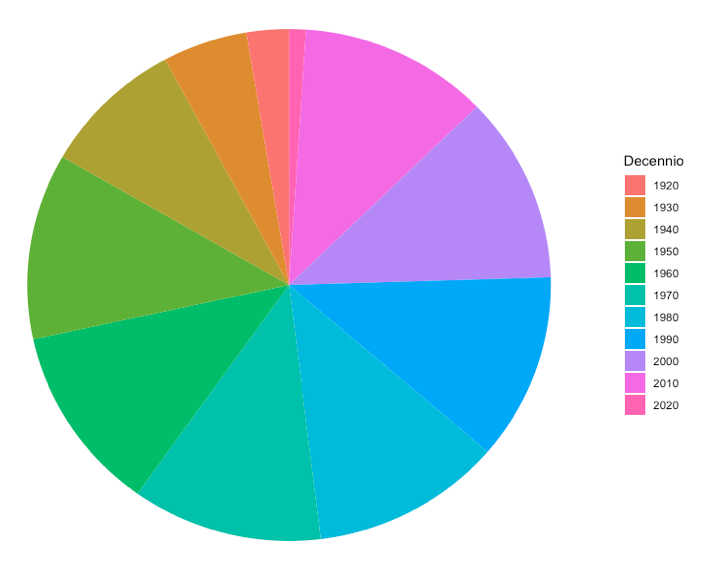
\includegraphics[width=0.7 \linewidth]{fig1.png}
    \label{fig:fig1}
    \caption{Aerogramma per la visualizzazione delle frequenze relative dei decenni.}
\end{figure}
Si è poi proceduto a verificare l'esistenza di una connessione fra questa nuova variabile e il grado di popolarità dei brani, eseguendo un test Chi-quadrato, cui ipotesi nulla
\begin{equation}
  H_0:\chi^2=0  
\end{equation}
coincide con l'indipendenza fra i due fenomeni. L'indice di associazione $\chi^2$ è dunque calcolato con $(k_1-1)(k_2-1)=990$ gradi di libertà, con $k_1=11$ e $k_2=100$ i rispettivi conteggi delle modalità. Fissato un livello di significatività $\alpha=0.05$, è stato ottenuto un valore \textit{pvalue} considerevolmente inferiore ad $\alpha$\footnote{Il \textit{pvalue} in questione è inferiore alla soglia $2.2\bullet10^{-16}$.}, portando a rifiutare, con confidenza al 95\%, l'ipotesi nulla di indipendenza fra il decennio di uscita della traccia e il proprio grado di popolarità. Ciò significa che le distribuzioni condizionali della popolarità variano in base alla decade considerata, come visibile in Figura \ref{fig:fig2}. 
\begin{figure}[H]
    \centering
    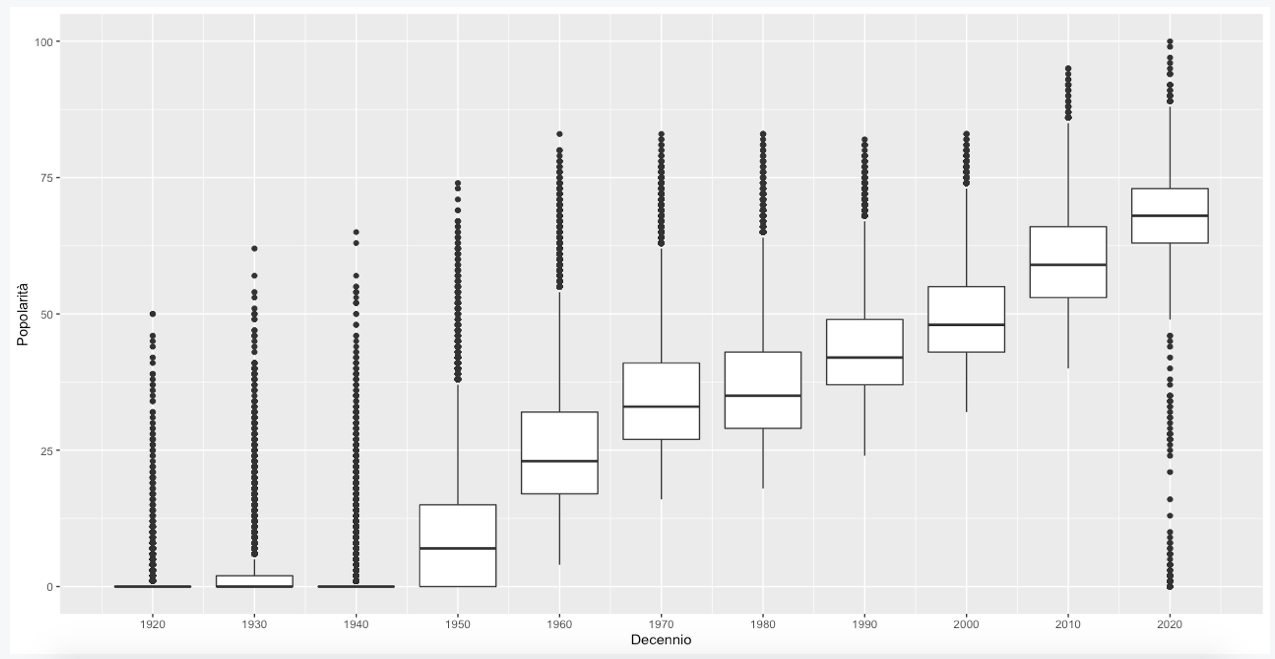
\includegraphics[width=1 \linewidth]{fig2.png}
    \label{fig:fig2}
    \caption{\textit{BoxPlot} condizionati per la visualizzazione delle distribuzioni condizionate di popolarità in base al decennio esaminato.}
\end{figure}
La natura di questa dipendenza statistica viene approfondita mediante test ANOVA, basato sull'ipotesi nulla di uguaglianza di tutte le popolarità medie, ovvero sull'ipotesi che le osservazioni di popolarità relative a ciascun decennio provengano da popolazioni che seguono una distribuzione normale con varianza e media pari. Si punta pertanto a verificare l'ipotesi alternativa, cioè che la media di almeno un gruppo differisca dalle altre, dimostrando che il fattore condizionante della decade ha un'influenza sulla popolarità. La statistica test è associata a 10 gradi di libertà e, fissato un livello di significatività $\alpha=0.05$, è stato ottenuto un valore \textit{pvalue} ancora una volta nettamente inferiore ad $\alpha$, causando il rifiuto dell'ipotesi nulla di uguaglianza delle popolarità medie per decennio e confermando, con una confidenza al 95\%, la presenza di una forte relazione fra queste due variabili. Osservando la Figura, è possibile riscontrare, almeno visivamente, una tendenza comprensibile: la preferenza degli utenti a livello aggregato appare quasi perfettamente ordinata per "novità" del brano.
\subsection*{Variabile \textit{Explicit}}
Un fenomeno, al contrario, distribuito in maniera sbilanciata è la presenza di contenuto esplicito nel testo: la frequenza percentuale delle tracce non esplicite è pari al 91.51\% (Figura \ref{fig:fig3}) e il suo indice di Gini normalizzato conferma la bassa mutabilità: $\sim$0.311. 
\begin{figure}[H]
    \centering
    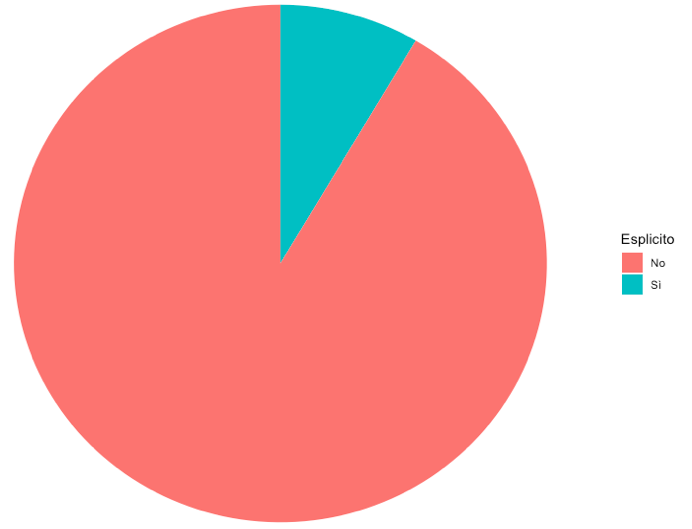
\includegraphics[width=0.7 \linewidth]{fig3.png}
    \label{fig:fig3}
    \caption{Aerogramma per la visualizzazione delle rispettive frequenze relative di contenuto esplicito e non esplicito.}
\end{figure}  
\subsection*{Variabile \textit{Mode}}
\subsection*{Variabile \textit{Key}}
%------------------------------------------------
\section{Analisi dei caratteri quantitativi}\label{cquant}
\subsection*{Variabile \textit{Acousticness}}
\subsection*{Variabile \textit{Danceability}}
\subsection*{Variabile \textit{Duration}}
\subsection*{Variabile \textit{Energy}}
\subsection*{Variabile \textit{Instrumentalness}}
\subsection*{Variabile \textit{Liveness}}
\subsection*{Variabile \textit{Loudness}}
\subsection*{Variabile \textit{Speechiness}}
\subsection*{Variabile \textit{Tempo}}
\subsection*{Variabile \textit{Valence}}
\subsection*{Variabile \textit{Popularity}}
\subsection{Correlazioni lineari}
%------------------------------------------------
\section{Regressione semplice}

%------------------------------------------------
\section{Regressione multipla}
\subsection{Previsione di \textit{Popularity}}
\subsection{Previsione di \textit{Valence}}
%------------------------------------------------
\section{Conclusioni}

%------------------------------------------------
\section*{Codice}
L'intero codice, implementato con linguaggio \texttt{R}, è disponibile al link: \href{https://github.com/RCrvro/Foundation-of-Prob.-and-Stat.---Final-Project/blob/master/codice.R}{\texttt{github.com/RCrvro/codice.R}}.
%----------------------------------------------------------------------------------------
%	REFERENCE LIST
%----------------------------------------------------------------------------------------

\clearpage

\phantomsection
\bibliographystyle{unsrt}
\begin{thebibliography}{9}


\end{thebibliography}
%----------------------------------------------------------------------------------------

\end{document}

